\hypertarget{part-2-image-4}{%
\section{Part 2, Image 4}\label{part-1-design-2}}

\centering


\hypertarget{description}{%
	\subsubsection{Description}\label{description}}

\begin{description}
	\item[Image:]
	\item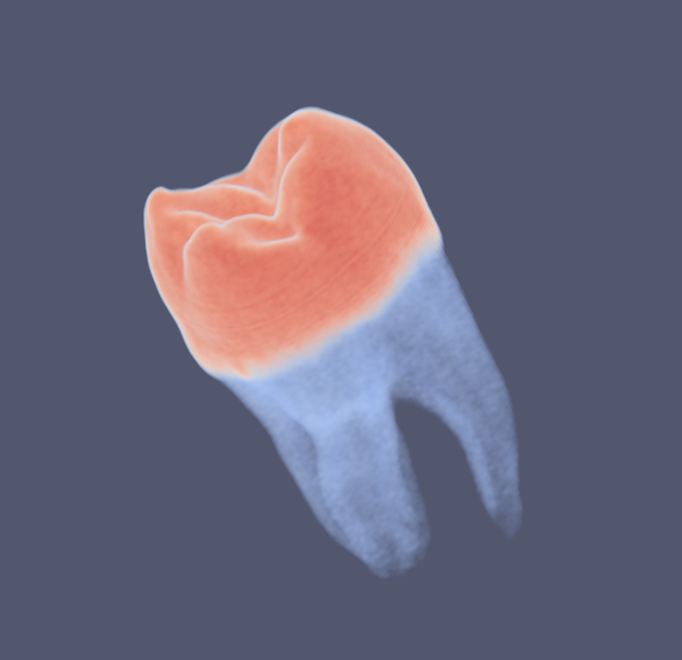
\includegraphics[width=9cm]{Tooth2.png}

	\item[Tool:]
	Paraview
	\item[Visual Mappings:]
	\begin{itemize}
		\tightlist
		\item[ ]
	\end{itemize}
	\begin{itemize}
		\tightlist
		\item
		\textbf{mapping 1}: Answer
	\end{itemize}
	
	\begin{itemize}
		\tightlist
		\item
		\textbf{mapping 2}: Answer
	\end{itemize}
	\item[Data Preparation:] Answer
	\item[Unique Observation:]
	At datapoint 948.195 is where the transition from the root to the actual tooth. This is the white strip in the image.
	
\end{description}